\documentclass[11pt,a4paper]{article}


\usepackage{amssymb,amsmath,amsfonts}    %ams
\usepackage{wasysym} %des symboles
%\usepackage{a4wide}
\usepackage[tmargin=1in,bmargin=1in,lmargin=.75in,rmargin=.75in]{geometry}
\usepackage{graphicx}
%\usepackage{pstricks}
%\usepackage{multido}
\usepackage{verbatim}
\usepackage{enumerate}
\usepackage{tikz}
\usetikzlibrary{calc,positioning,backgrounds}

\usepackage[utf8]{inputenc} 
%\usepackage[T1]{fontenc}
\usepackage{listings}

\newcommand{\R}{{\mathbb R}}   % reals
\newcommand{\Q}{{\mathbb Q}}   % rationals
\newcommand{\N}{{\mathbb N}}   %natural numbers
\newcommand{\Z}{{\mathbb Z}}    %integers
\renewcommand{\P}{{\mathbb P}}   %primes
\newcommand{\F}{{\mathbb F}}

\newcommand\cc{{\cal C}}
\newcommand{\cw}{{\cal W}}



\newtheorem{theorem}{Theorem}
\newtheorem{cor}{Corollary}
\newtheorem{example}{Example}
\newtheorem{lemma}{Lemma}
\newtheorem{newcommandi}{Definition}


\newcommand{\proof}{\noindent {\bf Proof.\ \ }}

\newcommand{\qed}{\hfill $\square$}


\newcommand{\card}[1]{\vert #1 \vert}

%\newcommand{\qed}{\hspace*{\fill} $\Box$ \bigskip }


%\renewcommand{\thefootnote}{\Alph{footnote}}
\usepackage{fancybox}
\usepackage[french]{babel}
%\usepackage{fullpage}
\usepackage{multicol}
\setlength{\columnseprule}{0.2pt}
\setlength{\columnsep}{16pt}
\usepackage{fancyhdr} % personalisation tete/pied de page
%\pagestyle{fancy}







\usepackage{hyperref}

%\addtolength{\headheight}{50pt}

\setlength{\parindent}{0pt}

\title{Fiche 5.1 : complexité des structures de données}
\author{BUT Informatique\\
IUT de Vélizy\\
}
\date{}


%\catcode`\_=12 %for escaping underscore

\newcommand{\ww}[1]{\textcolor{white}{#1}}

\newcommand{\code}[1]{%
    \begin{center}
        \tt #1
        \vskip .2cm
        {\tt
            \lstinputlisting[frame=single]{#1}
        }
    \end{center}
}


\usepackage{marginnote}

\usepackage{fancyvrb} % Verbatim avancé

\lstdefinestyle{customc}{
    belowcaptionskip=1\baselineskip,
    breaklines=true,
    frame=single,
    xleftmargin=2cm,
    language=C,
    showstringspaces=false,
    showspaces=false,
    basicstyle=\ttfamily
}


\newcommand{\reflexion}{\hspace{-1.2cm} 
\includegraphics[width=1cm]{reflexion.jpg} \vskip -.8cm}
%\newcommand{\checkbox}{
\includegraphics[width=.5cm]{checkbox.jpg} }
\newcommand{\checkbox}{$\square$ \smallskip}


%%environement pour les icones avec decalage
\newenvironment{icone}[1]{%
    \hskip -.8cm
\begin{tabular}{c|c}
    \hspace{.03\textwidth} \includegraphics[width=.07\textwidth]{#1} & 
\begin{minipage}{.85\textwidth}
}{%
\end{mieonipage}
\end{tabular}
}





\newcounter{exo} \setcounter{exo}{0}
\newenvironment{action}{%
    \begin{enumerate}[\numerotation] \addtocounter{exo}{-1}%
        }{%
    \end{enumerate}
}

%environement pour liste avec checkbox avec compteur
\newcommand{\numexoa}{\theexo \addtocounter{exo}{1}}
\newcommand{\numerotation}{\checkbox \smallskip \numexoa.}

%%environement de validation
\newenvironment{validation}{%
\smallskip
\begin{tabular}{c|c}
    \hspace{.03\textwidth} 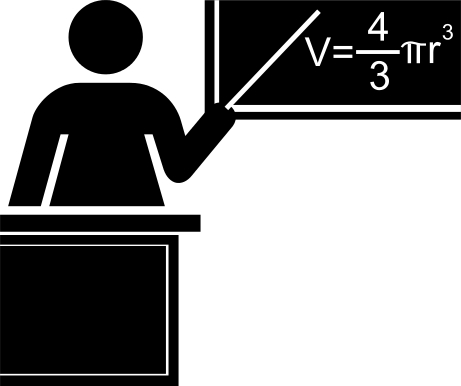
\includegraphics[width=.07\textwidth]{teacher.jpg} & 
\begin{minipage}{.85\textwidth}
}{%
\end{minipage}\\
\hline
\end{tabular}
}


%pour les fichiers c et dossiers
\newcounter{exoo} \setcounter{exoo}{0}
\newcommand{\numexo}{\theexoo}
\newcommand{\repexo}{{\tt exo\_\numexo}}
\newcommand{\exoplus}{\addtocounter{exoo}{1}}




\begin{document}
\maketitle





\thispagestyle{empty}

% \setcounter{section}{-1}
% \section{Introduction}
Dans ce TP, vous allez procéder aux mêmes {\bf mesures de performance} et aux mêmes {\bf affichages graphiques} que dans le TP précédent. Mais cette fois-ci, votre travail portera sur l'étude des deux principales structures de données natives de python: {\tt list} et {\tt dict}.\ 

En effet, nous allons nous poser les questions suivantes (et y répondre empiriquement):
\begin{itemize}
  \item le {\bf temps de construction} d'une liste et d'un dictionnaire sont-ils les mêmes?
  \item l'{\bf accès} à un enregistrement dans une liste ou un dictionnaire sont-ils aussi rapides? Dépendent-ils de la taille du dictionnaire?
  \item la {\bf recherche} dans une liste ou un dictionnaire, via la fonction native {\tt in}, offrent-ils les mêmes performances?
\end{itemize}

{\bf Objectif}: savoir choisir avec discernement les structures que vous utilisez dans vos programmes.\ 

Vous travaillerez dans un fichier de votre choix, fonctionnant sur le même principe que dans le TP précédent. Inutile d'écrire des fonctions, nous allons tout écrire dans un main.

\subsection*{Préparatifs}
\begin{action}
\item {\bf Intervalle} Définissez des constantes {\tt STEP}, {\tt NBSTEPS} et {\tt REP} indiquant respectivement le pas de construction des structures, le nombre d'étapes, et le nombre de répétitions. Exemple, si {\tt STEP=100}, {\tt NBSTEPS=200} et {\tt REP=50}, cela signifie qu'on va manipuler des structures de taille 100 à 20000 par pas de 100, et qu'on répètera les tests 50 fois afin de stabiliser les mesures.
\item {\bf Boucle principale} Construisez une liste {\tt lx} qui contienne toutes les tailles de structure que nous allons créer (en utilisant {\tt STEP} et {\tt NBSTEPS}, donc). Lancez ensuite une grande boucle {\tt for} où {\tt n} parcourt cette liste {\tt lx}. Ce sera notre boucle principale.
\end{action}

\subsection*{Construction d'une structure}
\begin{action}
\item {\bf Construction de liste }} Vous allez mesurer le temps de construction d'une liste {\tt l} de taille {\tt n}, contenant les entiers de {\tt 0} à {\tt n-1}, dans l'ordre. Récupérez les temps de construction dans une liste {\tt perfConstList} que vous utiliserez, comme dans le TP précédent, pour afficher un joli graphique.
\item {\bf Construction de dictionnaire} De la même manière, on construit un dictionnaire contenant {\tt n} enregistrements de la forme {\tt i:i} avec {\tt i} compris entre {\tt 0} et {\tt n-1}. On mesure le temps de construction et on le stocke dans une liste {\tt perfConstDict}, puis on crée le graphique associé.
\item {\bf Les tests} Testez votre programme avec {\tt STEP=200}, {\tt NBSTEPS=200}. La constante {\tt REP} n'et pas utilisée pour le moment.
\item {\bf Conclusions} Qu'en concluez-vous?
\end{action}

\subsection*{Accès à une structure}
\begin{action}
\item {\bf Accès aux listes} Dans la grande boucle précédente, nous allons ajouter, derrière les constructions, les mesure d'accès aux structures de taille variable que vous avez précédement créées. Ecrivez une boucle qui effectue {\tt REP} tours, et, dans cette boucle, écrit simplement un 0 dans la case d'indice {\tt len(l)//2} de la liste précédement créée. Vous calculerez le temps moyen mesuré pour cet accès et l'ajouterez dans une liste {\tt perfAccList}.
\item {\bf Accès aux dictionnaires} Même chose avec les dictionnaires: vous écrirez un 0 dans l'enregistrement d'indice {\tt len(d)//2} du dictionnaire et stockerez le temps moyen pour cet accès dans une liste {\tt perfAccDict}.
\item {\bf Les tests} Testez votre programme global, en fixant {\tt REP=500}, tracez les graphiques.
\item {\bf Conclusions} Que concluez-vous?
\end{action}

\subsection*{Recherche dans une structure}
\begin{action}
\item {\bf Recherche dans une liste} Toujours dans la boucle principale, vous allez mesurer le temps requis pour {\tt REP} recherches dans la liste créée précédement. Vous rechercherez un nombre qui n'y figure pas: -1. Pour utiliser la fonction native {\tt in} de python, vous avez juste à écrire {\tt -1 in l}. Stockez les performances moyennes dans {\tt perfRechList}.
\item {\bf Recherche dans un dictionnaire} Même chose dans les dictionnaires. Vous stockerez les performances dans une liste {\tt perfRechDict}.
\item {\bf Les tests} Lancez vos tests et graphiques.
\item {\bf Conclusions} Qu'en concluez-vous?
\end{action}


\end{document}
